\section{Dynamic Screening and UOT problem}
\subsection{Screening for UOT}

For UOT problem \ref{eq:uot}, we could get its dual form. 
\begin{lem}(Dual form of UOT problem)
\begin{equation}
\begin{split}
-d^*(-\theta) - g^*(X^{\tranT}\theta)& = -\frac{1}{2}\|\theta\|_2^2-y^{\tranT}\theta \\
 \mathbf{s.t.} \quad \forall i \quad x_i^{\tranT}\theta -\lambda c_i &\leq 0
 \end{split}
 \label{eq:uotdual}
\end{equation}
\end{lem}
The equation indicate a dual feasible area constructed by many dual constraints, the optimal solution is inside the constraints.\\
From the KKT condition, we can make sure that, for the optimal primal solution $\hat{t}$:
\begin{thm} (Screening) For the dual optimal solution $\hat{\theta}$, we have the following relationship:
 \begin{equation}
\begin{split}
x_i^{\tranT}\hat{\theta} -\lambda c_i  \left\{
\begin{aligned}
< 0 \quad& \Rightarrow \hat{t}_i = 0\\
= 0 \quad& \Rightarrow \hat{t}_i \geq 0
\end{aligned}
\right.
 \end{split}
 \label{eq:screening}
\end{equation}
\end{thm}

As we do not know the information of $\hat{t}$ directly, we can construct an area $\mathcal{R}^{S}$ containing the $\hat{t}$, if

 \begin{equation}
\max_{t \in \mathcal{R}^S} x_i^{\tranT}\theta -\lambda c_i  < 0
\end{equation}
then we have:
 \begin{equation}
 x_i^{\tranT}\hat{\theta} -\lambda c_i  < 0
\end{equation}
which means the corresponding $\hat{t}_i = 0$, and can be screening out.

Now we start to construct the area containing $\hat{\theta}$, from \ref{circle} we know that, if we can find a $\tilde{\theta}$ inside the dual feasible area, we can construct a circle where $\hat{\theta}$ is.  
\begin{thm}
(UOT projection) For any any $\theta^k$, we can compute the projection $\tilde{\theta}^k$ onto the dual feasible area.
 \begin{equation}
		\tilde{\theta}_{i}=\left\{
	\begin{aligned}
			\theta_{i} - \max_{j \mod n =i}(\frac{\theta_{j_{1}}+\theta_{j_{2}}-c_j}{2}) &\quad 0\leq i<n\\
			\theta_{i} - \max_{in\leq j <i(n+1)}(\frac{\theta_{j_{1}}+\theta_{j_{2}}-c_j}{2}) & \quad n\leq i<2n
	\end{aligned}
	\right.
 \end{equation}
\end{thm}
	\begin{figure}[htbp]
	\begin{center}	
	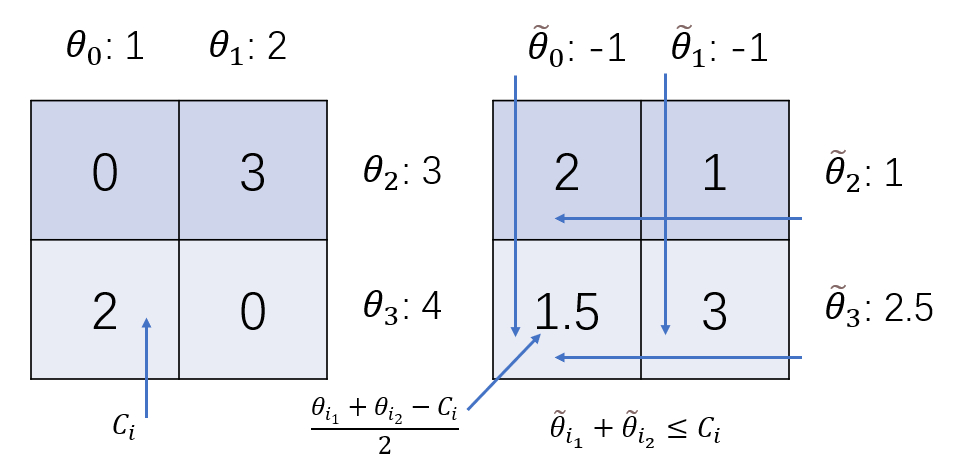
\includegraphics[width=0.8\hsize]{pic/shifting}
	\caption{Shifting on a 2$\times$2 matrix}
	\end{center}	
	\end{figure}

The intersection of the circle and the dual feasible area contain the $\hat{\theta}$, however, the multilinear constraints make it hard to compute the maximum for the problem, We design a relaxation method. which divide the constrains into two parts, then we are maximizing on the intersection of two hyperplane and a hyper-ball. 

\begin{thm}\label{area}(Screening Area for UOT) With the help of $\tilde{\theta}$, we can construct following area $\mathcal{R}^{S}$, and the optimal dual solution $\hat{\theta}$ must be inside the area.
 \begin{equation}
\begin{split} 
\mathcal{R}^S = \{ \theta \|
\begin{aligned}
 &\theta^{\tranT}X^A\beta - \lambda g^{A}\beta\leq 0 \\
  &\theta^{\tranT}X^B\beta - \lambda g^{B}\beta \leq 0\\
   &(\theta-\tilde{\theta})^{\tranT}(\theta-y)\leq 0\}
\end{aligned}
\end{split}
\label{eq:divide}
\end{equation}
\end{thm}
We devide the constraints into two group $A$ and $B$, we have $X^A +X^B=X$ and $g^A+g^B = g$
the computational process is in Appendix.A

\subsection{Screening Algorithms}

 \begin{algorithm}
 \caption{UOT Dynamic Screening Algorithm}
 \begin{algorithmic}[1]
 \renewcommand{\algorithmicrequire}{\textbf{Input:}}
 \renewcommand{\algorithmicensure}{\textbf{Output:}}
 \REQUIRE $t_0, S \in R^{n\times m}, S_{ij}=1$
 \ENSURE  $S$
  \STATE \text{Choose a solver for the problem.}
  \FOR {$t = 0 \text{ to } K$}
  \STATE $\text{Projection } \tilde{\theta} = \operatorname{Proj}(t^k)$ 
  \IF {($i \ne 0$)}
  \STATE $\textbf{break}$
  \ENDIF
    \STATE $\mathcal{R} \Leftarrow \mathcal{R}^S{(\tilde{\theta},t^k)}$
    \STATE $S \Leftarrow {S_{ij} = 0 \text{ if } \max_{\theta \in \mathcal{R}^S} {x_{k(i,j)}}^{\tranT}\theta <\lambda c_{k(i,j)} }$
    \FOR {$a  \in {A_{ij}\|A_{ij}=0}$}
    \STATE $t^k(i,j) \Leftarrow 0$
    \ENDFOR
    \STATE $t^{k+1} = \operatorname{update}(t^k)$
  \ENDFOR
  
 \RETURN $t^{K+1}, S $ 
 \end{algorithmic} 
 \end{algorithm}

screening method is irrelevent to the optimization solver you choose. We give the specific algorithm for $L_2$ UOT problem to show the whole optimization process.\\











































